\documentclass{beamer}
\usetheme{default} % very plain
\setbeamertemplate{navigation symbols}{} % remove nav symbols
\setbeamertemplate{footline}[frame number]

% SET THE LANGUAGE TO ENGLISH %
\usepackage[english]{babel}

% GRAPHICS CONFIGURATION %
\usepackage{graphicx}
\graphicspath{{images/}}

% HYPERLINK CONFIGURATION %
\usepackage{hyperref}
\hypersetup{
  colorlinks=true,
  linkcolor=black,
  filecolor=blue,
  citecolor=blue,
  urlcolor=blue,
}

% CODE LISTINGS WITH SYNTAX HIGHLIGHTING %
% See example: https://www.overleaf.com/learn/latex/Code_Highlighting_with_minted
% Restart the counter on every chapter
\usepackage[chapter,newfloat]{minted}
\setminted{
  linenos, % Show line numbers
  numbers=left, % Show the line numbers on the left
  xleftmargin=0.5cm, % Add marging so that the line numbers show up
  breaklines, % Wrap lines if necessary
  autogobble, % Remove whitespace in front of the code
  frame=lines, % Use lines to create a frame
  framesep=2mm, % Separation of the frame from the actual code
  fontsize=\scriptsize % Use a tiny font size
}
% Define a new environment for inline Rust code
\newmintinline{Rust}{
  fontsize=\small
}

\title[Ipopt revisited: Strategies to solve edge cases]{Ipopt revisited: Strategies to solve edge cases}
\author{Horacio Lisdero Scaffino}
\date{May 21, 2026}

\AtBeginSection[]
{
  \begin{frame}{Agenda}
  \tableofcontents[currentsection]
  \end{frame}
}

\begin{document}

\begin{frame}
  \titlepage
\end{frame}

\begin{frame}{Agenda}
  \tableofcontents
\end{frame}

\section{A tour of Ipopt}

\begin{frame}{Ipopt: Interior Point OPTimizer}

  Popular open-source non-linear optimization package

  \vfill

  Bindings available for:

  \begin{itemize}
    \item AMPL (algebraic modeling language)
    \item Fortran
    \item GAMS (general algebraic modeling system)
    \item Julia
    \item Matlab / Scilab
    \item .NET languages: C\#, F\# and Visual Basic.NET
    \item Python (several wrappers available)
    \item R
    \item Rust
  \end{itemize}

\end{frame}

\subsection{History}

\begin{frame}{Ipopt: The origins}

  \begin{itemize}
    \item PhD thesis by Andreas Wächter in 2002 at Carnegie Mellon \cite{wachter2002interior}
    \item Since 2002 part of the COIN-OP foundation \cite{coinop_ipopt}
    \item Original implementation in Fortran 77 (1.x and 2.x), now deprecated
    \item Open source since the start
    \item Benchmarked against KNITRO (1999) and LOQO (1999) \cite{byrd1999interior, vanderbei1999loqo}
  \end{itemize}

\end{frame}

\begin{frame}{Ipopt: Subsequent paper}

  \begin{itemize}
    \item Paper by Wächter and Biegler in 2006 \cite{wachter2006implementation}
    \item More focused on the central algorithm of Ipopt
    \item Features described more in detail
          \begin{itemize}
            \item Feasibility restoration phase,
            \item Inertia correction,
            \item Various heuristics...
          \end{itemize}
    \item More benchmarks: CUTEr test set \cite{gould2003cuter}
  \end{itemize}

\end{frame}

\begin{frame}{Ipopt: C++ version}

  \begin{itemize}
    \item IBM Research decided to invest in an open source re-write of Ipopt in C++
    \item With the help of Carl Laird, the code was re-implemented from scratch \cite{IpoptDocs}
    \item 3.x published in Aug 2005
    \item It is still actively developed on GitHub
  \end{itemize}

\end{frame}

\subsection{Techniques applied}

\begin{frame}{Ipopt: Summary of applied techniques}

  \begin{itemize}
    \item \fbox{Primal-dual interior-point method} with filter line-search globalization
    \item \fbox{Sparse symmetric KKT solves} with inertia monitoring/correction
    \item Inertia correction and regularization to obtain the proper search direction
    \item Feasibility restoration phase for difficult or infeasible iterates
    \item Second-order correction steps to reduce Maratos-type effects
    \item Practical heuristics for robustness and faster performance
  \end{itemize}

\end{frame}

\begin{frame}{Interior Point Methods: Intro}
  \vspace{-2.0em}

  \begin{align}
    \min_{x \in \mathbb{R}^n}\quad & \varphi_\mu(x) := f(x) - \mu \sum_{i=1}^n \ln\!\bigl(x^{(i)}\bigr) \\
    \text{s.t.}\quad               & c(x) = 0                                                           \\
    \quad                          & x \ge 0
  \end{align}

  We recover the Karush-Kuhn-Tucker (KKT) conditions for $\mu = 0$:

  \vspace{-1.0em}

  \begin{align}
    \nabla f(x) + \nabla c(x)\lambda - z       & = 0                                    \\
    c(x)                                       & = 0                                    \\
    XZ e - \mu e                               & = 0                                    \\
    x, z \ge 0,\qquad \lambda \in \mathbb{R}^m & , \qquad z \in \mathbb{R}^n, \nonumber \\
    Z := \operatorname{diag}(z), e             & = (1,\dots,1)^T \nonumber
  \end{align}

  $n$: number of primal variables, $m$: number of equality constraints

\end{frame}


\begin{frame}{KKT system: Derivation}
  \vspace{-2.0em}

  \[
    F_\mu(x,\lambda,z) =
    \begin{bmatrix}
      \nabla f(x) + \nabla c(x)\lambda - z \\
      c(x)                                 \\
      XZe - \mu e
    \end{bmatrix} = 0
  \]

  Iteratively solve using Netwon's method:

  \begin{itemize}
    \item Fix a starting point $(x_k, \lambda_k, z_k)$,
    \item Calculate the deltas for each dimension $(d_k^x, d_k^\lambda, d_k^z)$
    \item Use the deltas to move to $(x_{k+1}, \lambda_{k+1}, z_{k+1})$ (more later)
  \end{itemize}

  \[
    F_{\mu_j}(x_k,\lambda_k,z_k) + \nabla F_{\mu_j}(x_k,\lambda_k,z_k) (d_k^x, d_k^\lambda, d_k^z)^T = 0
  \]


  The term $\nabla F_\mu(x,\lambda,z)$ is a 3x3 matrix.

  It is the Jacobian of the vector field.

  We can move $F_\mu(x,\lambda,z)$ to the other side to get the form $A x = b$.

\end{frame}

\begin{frame}{KKT system: Matrix form}
  \vspace{-1.0em}

  \begin{align*}
    \begin{bmatrix}
      W_k   & A_k & -I  \\
      A_k^T & 0   & 0   \\
      Z_k   & 0   & X_k
    \end{bmatrix}
    \begin{bmatrix}
      d_k^x       \\
      d_k^\lambda \\
      d_k^z
    \end{bmatrix}
                             & =
    -
    \begin{bmatrix}
      \nabla f(x_k) + A_k \lambda_k - z_k \\
      c(x_k)                              \\
      X_k Z_k e - \mu_j e
    \end{bmatrix}                                        \\[0.8em]
    \text{where}\qquad
    A_k                      & := \nabla c(x_k),                               \\
    W_k                      & := \nabla^2_{xx}\mathcal{L}(x_k,\lambda_k,z_k), \\
    \mathcal{L}(x,\lambda,z) & := f(x) + c(x)^T\lambda - z.
  \end{align*}

  But this system can be further simplified!

  Multiply out the third equation:

  \vspace{-1.0em}
  \begin{align*}
    Z_k d_k^x + X_k d_k^z      & = \mu_j e - X_k Z_k e    \\
    d_k^z = \mu_j X_k^{-1} e - & z_k - X_k^{-1} Z_k d_k^x \\
    \Sigma_k                   & := X_k^{-1} Z_k
  \end{align*}

\end{frame}

\begin{frame}{KKT system: Symmetric matrix form}
  \vspace{-2.0em}

  Now $d_k^z$ only appears in the first equation as $-I d_k^z = - d_k^z$ which we move to the other side:

  \vspace{-1.0em}
  \begin{align*}
    W_k d_k^x + A_k d_k^\lambda              & = - (\nabla f(x_k) + A_k \lambda_k - z_k) + d_k^z      \\
    W_k d_k^x + A_k d_k^\lambda              & = - (\nabla f(x_k) + A_k \lambda_k - z_k) +            \\
                                             & \qquad + \mu_j X_k^{-1} e - z_k - \Sigma_k d_k^x       \\
    (W_k + \Sigma_k) d_k^x + A_k d_k^\lambda & = - (\nabla f(x_k) + A_k \lambda_k - \mu_j X_k^{-1} e) \\
    (W_k + \Sigma_k) d_k^x + A_k d_k^\lambda & = - (\nabla \varphi_{\mu_j}(x_k) + A_k \lambda_k)
  \end{align*}

  Reconstructing the system, we get:

  \begin{equation}
    \begin{bmatrix}
      W_k + \Sigma_k & A_k \\
      A_k^T          & 0   \\
    \end{bmatrix}
    \begin{bmatrix}
      d_k^x       \\
      d_k^\lambda \\
    \end{bmatrix}
    =
    -
    \begin{bmatrix}
      \nabla \varphi_{\mu_j}(x_k) + A_k \lambda_k \\
      c(x_k)
    \end{bmatrix}
  \end{equation}

\end{frame}

\begin{frame}{KKT system: Important considerations}
  \vspace{-2.0em}

  \begin{equation*}
    \begin{bmatrix}
      W_k + \Sigma_k & A_k \\
      A_k^T          & 0   \\
    \end{bmatrix}
    \begin{bmatrix}
      d_k^x       \\
      d_k^\lambda \\
    \end{bmatrix}
    =
    -
    \begin{bmatrix}
      \nabla \varphi_{\mu_j}(x_k) + A_k \lambda_k \\
      c(x_k)
    \end{bmatrix}
  \end{equation*}

  \begin{itemize}
    \item Symmetric system
    \item Matrix in top-left block projected onto the null space of the constraint Jacobian $A_k^T$ is positive definite
    \item If $A_k$ does not have full rank, the iteration matrix is singular and a solution may not exist
  \end{itemize}

  Solve instead the following system with \textbf{inertia correction} for some $\delta_w, \delta_c \ge 0$:

  \begin{equation*}
    \begin{bmatrix}
      W_k + \Sigma_k + \delta_w I & A_k \\
      A_k^T          & - \delta_c I  \\
    \end{bmatrix}
    \begin{bmatrix}
      d_k^x       \\
      d_k^\lambda \\
    \end{bmatrix}
    =
    -
    \begin{bmatrix}
      \nabla \varphi_{\mu_j}(x_k) + A_k \lambda_k \\
      c(x_k)
    \end{bmatrix}
  \end{equation*}

\end{frame}

\section{An attempt of a simple IPM algorithm}

\begin{frame}{Introduction}

  I wanted to play around with code and not just present equations

  \begin{flushright}
    \scriptsize and thus produce some nice visualizations :)
  \end{flushright}

  \vfill
  \pause

  I wanted to see if optimization in pure Rust is possible

  \begin{flushright}
    \scriptsize memory safety, performance, modern language for low-level applications, ...
  \end{flushright}

  \vfill
  \pause

  I wanted to contribute something back to the community,

  \begin{flushright}
    \scriptsize i.e, \textbf{not} throw away the Python code 1 week after the seminar
  \end{flushright}

  \vfill

\end{frame}

\begin{frame}{The original plan}

  \begin{columns}[T]
    \begin{column}{0.5\textwidth}
      \begin{enumerate}
        \item Select the most popular optimization package
        \item Implement a simple interior-point method
        \item Compare it with Ipopt
        \item Profit!
      \end{enumerate}
    \end{column}

    \begin{column}{0.5\textwidth}
      \centering
      
\includegraphics[width=\textwidth]{obama-medal.jpg}
    \end{column}
  \end{columns}

\end{frame}

\begin{frame}{argmin}


  \centering
  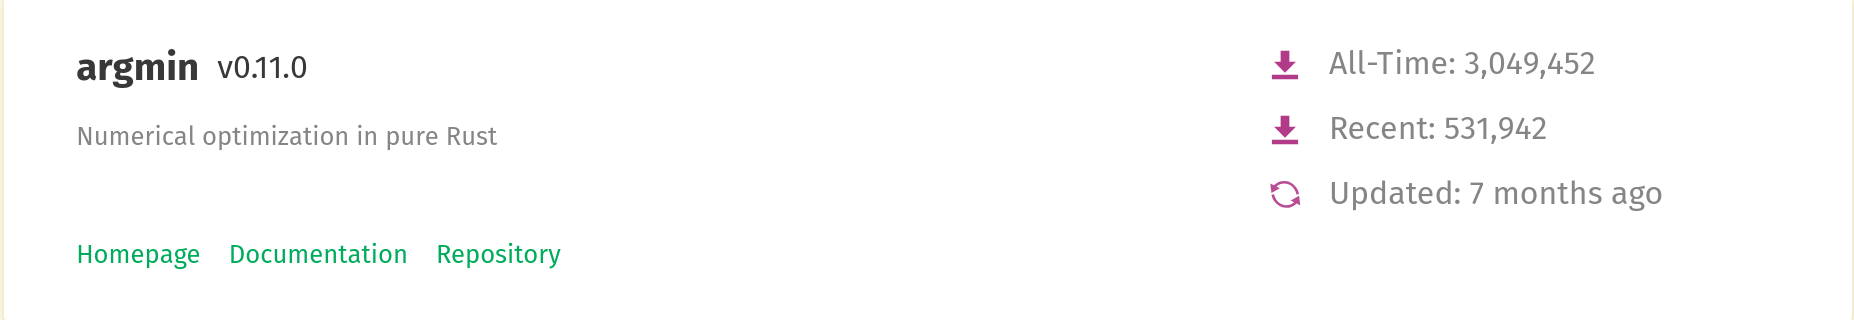
\includegraphics[width=\textwidth]{argmin-crate.png}

  \vfill

  \tiny Website \cite{argmin-rs}
  \centering
  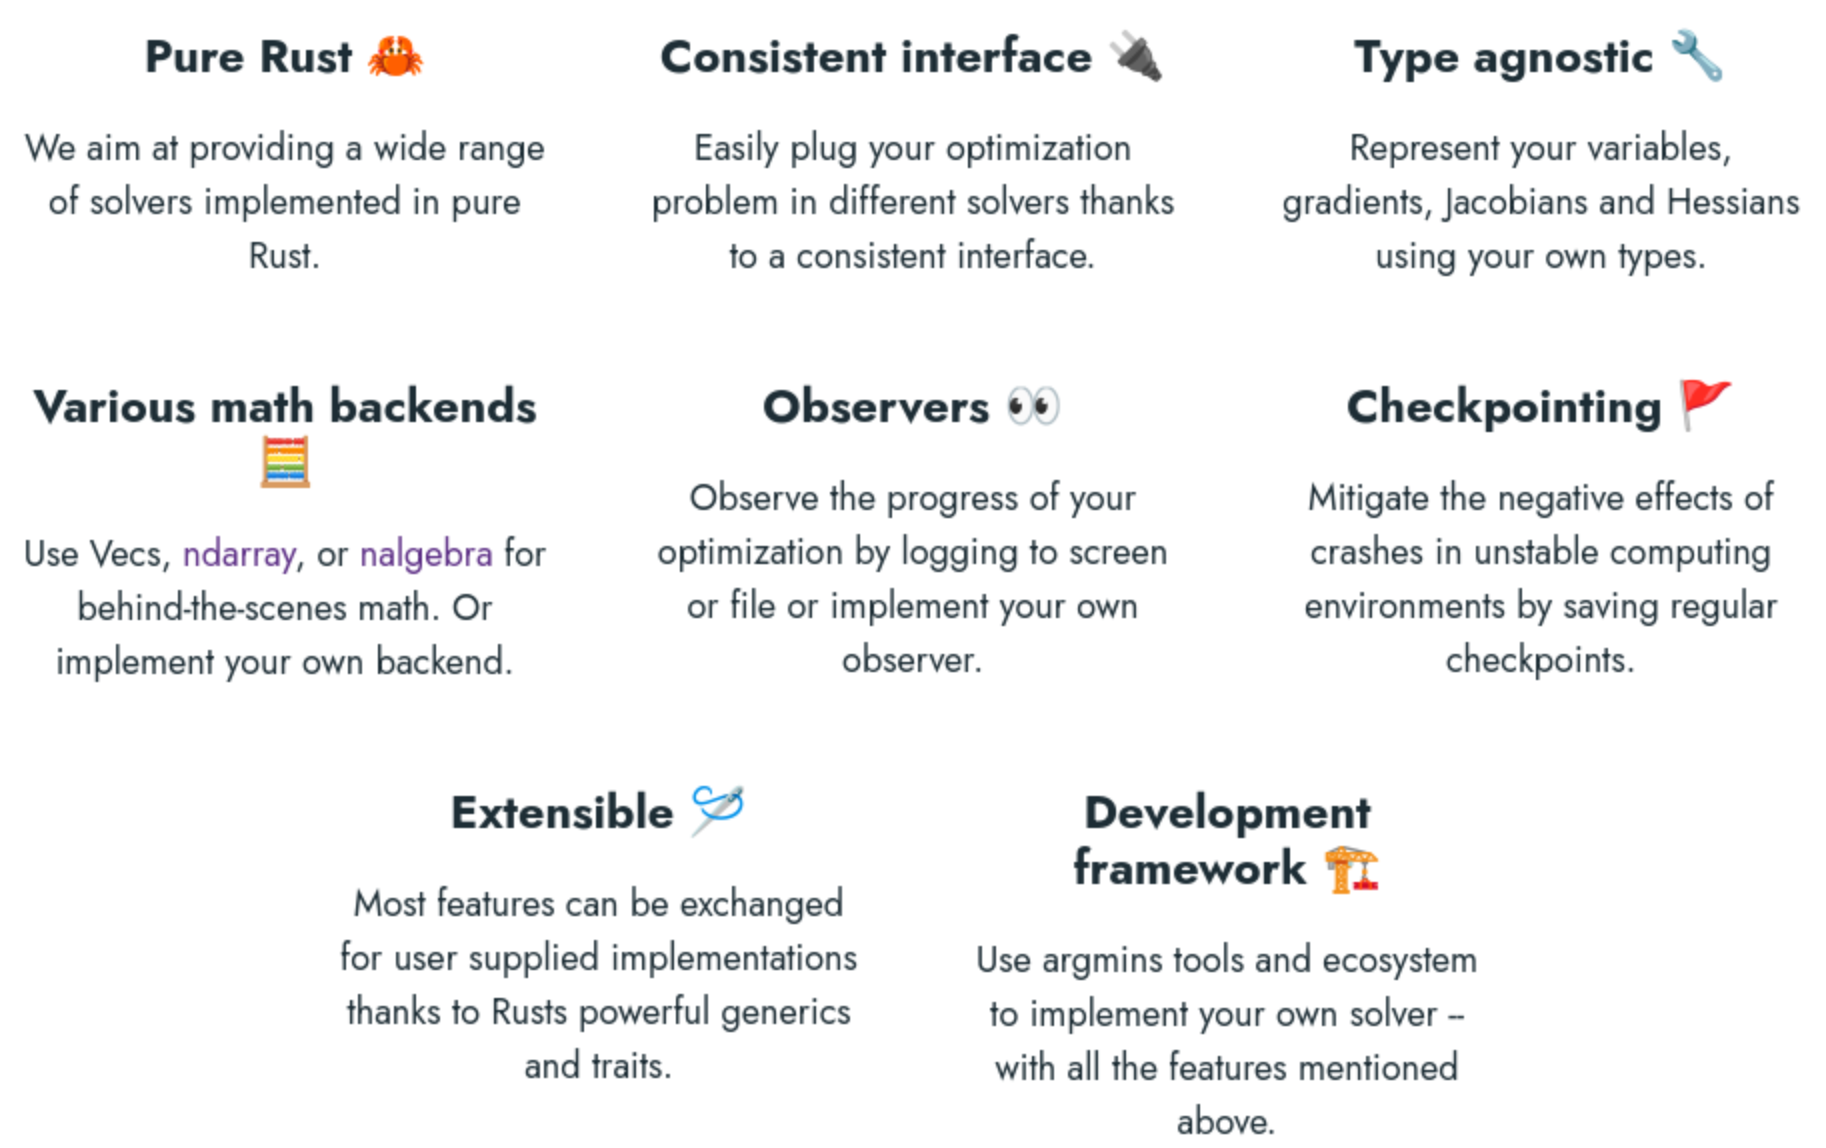
\includegraphics[width=\textwidth]{argmin-features.png}

  \vfill

  \tiny discarded several libraries: dealt only with LP (\texttt{good\_lp}), used novel algorithms (\texttt{clarabel}), or were too small (\texttt{interiors})

\end{frame}

\begin{frame}[fragile]{argmin: Code example}

  \begin{listing}
    \begin{minted}[fontsize=\tiny, frame=none]{Rust}
        impl<O, P, G, H, F> Solver<O, IterState<P, G, (), H, (), F>> for Newton<F>
        where
            O: Gradient<Param = P, Gradient = G> + Hessian<Param = P, Hessian = H>,
            P: Clone + ArgminScaledSub<P, F, P>,
            H: ArgminInv<H> + ArgminDot<G, P>,
            F: ArgminFloat,
        {
            fn next_iter(
                &mut self,
                problem: &mut Problem<O>,
                mut state: IterState<P, G, (), H, (), F>,
            ) -> Result<(IterState<P, G, (), H, (), F>, Option<KV>), Error> {
                let param = state.take_param().ok_or_else(argmin_error_closure!(
                    NotInitialized,
                    concat!(
                        "`Newton` requires an initial parameter vector. ",
                        "Please provide an initial guess via `Executor`s `configure` method."
                    )
                ))?;
                let grad = problem.gradient(&param)?;
                let hessian = problem.hessian(&param)?;
                let new_param = param.scaled_sub(&self.gamma, &hessian.inv()?.dot(&grad));
                Ok((state.param(new_param), None))
            }
        }
    \end{minted}
  \end{listing}

\end{frame}

\begin{frame}{Math backends}

  The math backend is implemented in a separate crate \texttt{argmin-math}

  \vfill

  It is trait-based: interfaces define the methods required from the linear algebra backend

  \vfill

  \begin{itemize}
    \item \texttt{nalgebra} \cite{nalgebra-rs}
    \item \texttt{faer} \cite{faer-rs}
  \end{itemize}

\end{frame}

\subsection{Challenges encountered}

\begin{frame}[fragile]{Add a solver}

  Add a trait:

  \begin{listing}
    \begin{minted}[fontsize=\tiny, frame=none]{Rust}
        pub trait ArgminLuSolve<T> {
            /// Solve linear system using LU decomposition.
            fn lu_solve(&self, rhs: &T) -> Result<T, Error>;
        }
    \end{minted}


  \end{listing}

  And the corresponding implementation:

  \begin{listing}
    \begin{minted}[fontsize=\tiny, frame=none]{Rust}
        impl<N, D, C, S> ArgminLuSolve<OMatrix<N, D, C>> for SquareMatrix<N, D, S>
        where
            N: ComplexField,
            D: Dim + DimMin<D, Output = D>,
            C: Dim,
            S: Storage<N, D, D>,
            DefaultAllocator: Allocator<N, D, D> + Allocator<N, D, C> + Allocator<N, D>,
        {
            #[inline]
            fn lu_solve(&self, rhs: &OMatrix<N, D, C>) -> Result<OMatrix<N, D, C>, Error> {
                let lu = LU::new(self.clone_owned());
                lu.solve(rhs).ok_or_else(|| LuSolveError {}.into())
            }
        }
    \end{minted}
  \end{listing}

\end{frame}

\begin{frame}[fragile]{No constraints?}

  \begin{listing}
    \begin{minted}[fontsize=\tiny, frame=none]{Rust}
        /// Defines equality constraints for a problem.
        ///
        /// It follows the form h(x) = (0, ... , 0), where h is a vector field.
        pub trait EqualityConstraint {
            /// Type of the parameter vector
            type Param;
            /// Type of the return value of the equality constraints
            type Output;

            /// Compute all equality constraints
            fn equality_constraint(&self, param: &Self::Param) -> Result<Self::Output, Error>;
        }
    \end{minted}
  \end{listing}

\end{frame}

\begin{frame}[fragile]{And their derivatives...}

  \begin{listing}
    \begin{minted}[fontsize=\tiny, frame=none]{Rust}
        /// Defines the Jacobian of the vector field representing the equality constraints for a problem.
        pub trait EqualityConstraintJacobian {
            /// Type of the parameter vector
            type Param;
            /// Type of the Jacobian
            type Jacobian;

            /// Compute the Jacobian of the equality constraints
            fn equality_constraint_jacobian(&self, param: &Self::Param) -> Result<Self::Jacobian, Error>;

            bulk!(equality_constraint_jacobian, Self::Param, Self::Jacobian);
        }
    \end{minted}
  \end{listing}

\end{frame}

\begin{frame}[fragile]{And the Hessian of the Lagrangian...}

  \begin{listing}
    \begin{minted}[fontsize=\tiny, frame=none]{Rust}
        pub trait LagrangianHessian {
            /// Type of the parameter vector
            type Param;
            /// Type of the multipliers associated with equality constraints
            type MultipliersEq;
            /// Type of the multipliers associated with inequality constraints
            type MultipliersIneq;
            /// Type of the Hessian
            type Hessian;

            /// Compute the Hessian of the Lagrangian
            fn lagrangian_hessian(
                &self,
                param: &Self::Param,
                multipliers_eq: &Self::MultipliersEq,
                multipliers_ineq: &Self::MultipliersIneq,
            ) -> Result<Self::Hessian, Error>;

            bulk!(
                lagrangian_hessian,
                Self::Param,
                Self::MultipliersEq,
                Self::MultipliersIneq,
                Self::Hessian
            );
        }
    \end{minted}
  \end{listing}

\end{frame}

\begin{frame}{And iteration state for NLP...}

  \scriptsize

  \begin{columns}[T,onlytextwidth]
    \column{0.48\textwidth}
    \begin{itemize}
      \item \texttt{param: Option<P>}
      \item \texttt{slacks: Option<S>}
      \item \texttt{best\_param: Option<P>}
      \item \texttt{best\_slacks: Option<S>}
      \item \texttt{cost: F}
      \item \texttt{best\_cost: F}
      \item \texttt{target\_cost: F}
      \item \texttt{grad: Option<G>}
      \item \texttt{lagrangian\_hessian: Option<LH>}
      \item \texttt{equality\_constraints: Option<EqC>}
      \item \texttt{inequality\_constraints: Option<IneqC>}
      \item \texttt{equality\_constraint\_jacobian: Option<EqCJ>}
      \item \texttt{inequality\_constraint\_jacobian: Option<IneqCJ>}
      \item \texttt{mu: Option<F>}
    \end{itemize}

    \column{0.48\textwidth}
    \begin{itemize}
      \item \texttt{lambda\_eq: Option<LambdaEq>}
      \item \texttt{lambda\_ineq: Option<LambdaIneq>}
      \item \texttt{alpha\_primal: Option<F>}
      \item \texttt{alpha\_dual: Option<F>}
      \item \texttt{inf\_pr: Option<F>}
      \item \texttt{inf\_du: Option<F>}
      \item \texttt{compl\_inf: Option<F>}
      \item \texttt{iter: u64}
      \item \texttt{last\_best\_iter: u64}
      \item \texttt{max\_iters: u64}
      \item \texttt{counts: HashMap<String, u64>}
      \item \texttt{counting\_enabled: bool}
      \item \texttt{time: Option<Duration>}
      \item \texttt{termination\_status: TerminationStatus}
    \end{itemize}
  \end{columns}

\end{frame}

\begin{frame}{Finally! IPM}


  \texttt{nalgebra\_backend.rs}: All the linear-algebra-specific logic for nalgebra, the only supported backend

  \vfill

  \texttt{linesearch.rs}: The custom backtracking linear search. The existing implementation could not be reused

  \vfill

  \texttt{iteration.rs}: A single iteration of the interior-point method

  \vfill

  \texttt{interiorpointmethod.rs}: The solver. The high-level management of the IPM algorithm.

\end{frame}

\subsection{Results}


\section{A tour of ripopt}

\begin{frame}{ripopt: A Rust re-write from February 2026}

  Coded in ~60/70 hs during the course of 6 weeks heavily relying on Claude Code \cite{kitchin_ripopt}.

  \vfill

  According to the benchmarks CUTEst and xxxx, it already beats Ipopt.

  \vfill

  Interesting insights into licensing issues and thought process documented in the repo.

\end{frame}

\section{Experiments}

\subsection{What can we learn}


\section{Conclusion}

\begin{frame}{Conclusion}

  Ipopt's performance can still be improved.

  \vfill

  Different methods complement each other: By combining them, edge cases can be solved more efficiently.

  \vfill

  Implementation of a state-of-the-art optimization package may be in the reach of modern AI agentic coding tools.

\end{frame}

\begin{frame}{Questions?}

  \textbf{Links}

  \scriptsize

  \vfill
  Presentation: \\
  \url{https://github.com/hlisdero/JMCS_Seminar_Applied_Optimization}

  \vfill
  Modified argmin: \\
  \url{https://github.com/hlisdero/argmin}

  \vfill
  ripopt: \\
  \url{https://github.com/jkitchin/ripopt}

  \vfill
  ipopt-rs: \\
  \url{https://github.com/elrnv/ipopt-rs}
\end{frame}

\section*{Bibliography}

\begin{frame}{Bibliography}
  \tiny
  \bibliographystyle{ieeetr}
  \bibliography{
    ./bibliography/Articles.bib,
    ./bibliography/Books.bib,
    ./bibliography/Repositories.bib,
  }
\end{frame}

\end{document}
